%%%%%%%%%%%%%%%%%%%%%%%%%%%%%%%%%%%%%%
% LaTeX poster template
% Created by Nathaniel Johnston
% August 2009
% http://www.nathanieljohnston.com/index.php/2009/08/latex-poster-template/
%%%%%%%%%%%%%%%%%%%%%%%%%%%%%%%%%%%%%%

\documentclass[final]{beamer}
\usepackage[scale=1.24]{beamerposter}
\usepackage{graphicx}			% allows us to import images

%-----------------------------------------------------------
% Define the column width and poster size
% To set effective sepwid, onecolwid and twocolwid values, first choose how many columns you want and how much separation you want between columns
% The separation I chose is 0.024 and I want 4 columns
% Then set onecolwid to be (1-(4+1)*0.024)/4 = 0.22
% Set twocolwid to be 2*onecolwid + sepwid = 0.464
%-----------------------------------------------------------

\newlength{\sepwid}
\newlength{\onecolwid}
\newlength{\twocolwid}
\newlength{\threecolwid}
\setlength{\paperwidth}{1189mm}
\setlength{\paperheight}{841mm}
\setlength{\sepwid}{0.024\paperwidth}
\setlength{\onecolwid}{0.1712\paperwidth}
\setlength{\twocolwid}{0.3664\paperwidth}
\setlength{\threecolwid}{0.5616\paperwidth}
\setlength{\topmargin}{-0.5in}
\usetheme{confposter}

%-----------------------------------------------------------
% Define colours (see beamerthemeconfposter.sty to change these colour definitions)
%-----------------------------------------------------------

\setbeamercolor{block title}{fg=ucdgold,bg=white}
\setbeamercolor{block body}{fg=black,bg=white}
\setbeamercolor{block alerted title}{fg=white,bg=ucdblue}
\setbeamercolor{block alerted body}{fg=black,bg=ucdblue!10}

%-----------------------------------------------------------
% Name and authors of poster/paper/research
%-----------------------------------------------------------

\title{Accurate Measurement of Bicycle Parameters}
\author{Jason K. Moore$^{*}$, Mont Hubbard$^{*}$, A. L. Schwab$^\dag$,
            J. D. G. Kooijman$^\dag$}
\institute
{
\centering
\begin{tabular}{cc}
$^*$ Mechanical and Aerospace Engineering, University of California, Davis
\quad
& $^\dag$ Laboratory for Engineering Mechanics, Delft University of Technology\\
e-mail: jkmoor@ucdavis.edu, mhubbard@ucdavis.edu
& e-mail: a.l.schwab@tudelft.nl, jodikooijman@gmail.com
\end{tabular}
}
%-----------------------------------------------------------
% Start the poster itself
%-----------------------------------------------------------
% The \rmfamily command is used frequently throughout the poster to force a serif font to be used for the body text
% Serif font is better for small text, sans-serif font is better for headers (for readability reasons)
%-----------------------------------------------------------

\begin{document}
\frame{
%\begin{frame}[t]

% Divide the frame into columns
\begin{columns}[t] % the [t] option aligns the column's content at the top

% Empty side column for spacing
\begin{column}{\sepwid}\end{column}	% empty spacer column

% First column with content
\begin{column}{\onecolwid}
  \begin{block}{Introduction}
    \rmfamily{
    Accurate estimates of a bicycle's physical parameters are required for
    realistic dynamic simulations and analysis. For the most basic models the
    geometry, mass, mass location and mass distribution of each rigid body
    must be measured. In particular, we are concerned with the measurement of
    the non-minimal set of 25 parameters required for the benchmark bicycle
    presented in~\cite{Meijaard2007}.
    The experimental methods described herein are based primarily on
    the work done in \cite{Kooijman2006} and \cite{Roland1971} but have been
    refined for improved accuracy and methodology. We measured the
    characteristics of six different bicycles, two of which were set up in two
    different configurations. We provide a total of eight different parameter sets
    that can be used with, but are not limited to, the benchmark bicycle model. The
    accuracies of all the measurements are presented along with a comparison of
    the linear characteristics of the eight bicycles.
    \\
    \scriptsize{\url{http://github.com/moorepants/PhysicalParameters}}
    }
  \end{block}
  \vskip2ex

  % Info about the model
  \begin{alertblock}{Whipple Bicycle Model}
    \small{\rmfamily{
    The linear unforced two degree-of-freedom, $\mathbf{q}$
    = [steer and roll], linear Whipple model takes the form:
    \begin{equation}
        \mathbf{M\ddot{q}}
        +v\mathbf{C}_1\mathbf{\dot{q}}
        +\left[g\mathbf{K}_0
        +v^2\mathbf{K}_2\right]\mathbf{q}
        =0
        \label{eq:canonical}
    \end{equation}
    where the entries to the $\mathbf{M}$, $\mathbf{C}_1$, $\mathbf{K}_0$ and $\mathbf{K}_2$
    matrices are combinations of 25 of the bicycle's physical parameters that
    include the geometry, mass, mass location and mass distribution of the four
    rigid bodies.
    }}
  \end{alertblock}

\end{column}

% Spacer column
\begin{column}{\sepwid}\end{column} % empty spacer column

% Second Column
\begin{column}{\twocolwid}
  \begin{block}{Accuracy}
    \rmfamily{
    Following in the vein of \cite{Roland1971} we used error propagation theory to
    calculate the accuracy of the estimates of 25 benchmark bicycle parameters.
    We first estimate
    the standard deviation of the raw measurements. If $x$ is a parameter and is a function of
    the raw measurements, $u,v,\ldots$, then $x$ is a random variable defined as
    $x=f(u,v,\ldots)$. The sample variance of $x$ is defined as
    \begin{equation}
        s_x^2 = s_u^2\left(\frac{\partial x}{\partial u}\right)^2 +
                s_v^2\left(\frac{\partial x}{\partial v}\right)^2 +
                2s_{uv}\left(\frac{\partial x}{\partial u}\right)\left(\frac{\partial x}{\partial v}\right)
                + \ldots
        \label{eqn:variance}
    \end{equation}
    where $s_u$ is the variance and $s_{uv}$ is the covariance. If $u$ and $v$ are uncorrelated then $s_{uv}=0$ but the cross correlations
    must be taken into account otherwise.
    }
  \end{block}
  \begin{columns}[t, totalwidth=\twocolwid]
      \begin{column}{\onecolwid}
          \begin{block}{Bicycles}
            \rmfamily{
            The six bicycles, chosen for both variety and convenience, are as follows:
            \emph{Batavus Browser}, a Dutch style city bicycle measured with and without
            instrumentation; \emph{Batavus Stratos
            Deluxe}, a Dutch style sporty city bicycle; \emph{Batavus Crescendo Deluxe} a
            Dutch style city bicycle with a suspended fork; \emph{Gary Fisher Mountain
            Bike}, a hardtail mountain bicycle; \emph{Bianchi Pista}, a modern steel frame
            track racing bicycle; and \emph{Yellow Bicycle}, a stripped-down aluminum frame
            road bicycle measured in two configurations, the second with the fork rotated
            in the headtube 180 degrees for larger trail.
            \\
            \begin{center}
                \begin{tabular}{ccc}
                    \includegraphics[width=0.333\onecolwid]{../../../images/browserIns_sub.jpg} &
                    \includegraphics[width=0.333\onecolwid]{../../../images/crescendo_sub.jpg} &
                    \includegraphics[width=0.333\onecolwid]{../../../images/fisher_sub.jpg}
                    \\
                    \includegraphics[width=0.333\onecolwid]{../../../images/pista_sub.jpg} &
                    \includegraphics[width=0.333\onecolwid]{../../../images/stratos_sub.jpg} &
                    \includegraphics[width=0.333\onecolwid]{../../../images/yellow_sub.jpg}
                \end{tabular}
            \end{center}
            }
          \end{block}
    \end{column}

    \begin{column}{\onecolwid}

  \begin{alertblock}{Eigenanalysis}
    \rmfamily{
    Distinct variation is apparent among the bicycles' eigenvalues. Frequency,
    damping, and the stable speed range can be compared to the physical
    differences of the bicycles. The bicycles also exhibit two complex root
    pairs at low speeds.
    }
    \\
    \begin{center}
      \includegraphics[width=.9\onecolwid]{../../../plots/Bike/eig_plot.pdf}
    \end{center}
    \rmfamily{
    Less variation is seen among the bicycles when a
    rigid rider is added, except in the stable speed ranges.
    }
    \\
    \begin{center}
      \includegraphics[width=.9\onecolwid]{../../../plots/BikeRider/eig_plot.pdf}
    \end{center}
  \end{alertblock}

    \end{column}
\end{columns}
\end{column}

% Spacer column
\begin{column}{\sepwid}\end{column} % empty spacer column

% The fourth column
\begin{column}{\onecolwid}
        \begin{block}{Measurements}
            \rmfamily{
            We estimated the wheel radii by measuring the distance traveled
            by the loaded wheels, the trail by directly measuring the fork
            offset and the wheelbase and headtube angle by direct measurement.
            We measured the mass of the four bodies (fork, frame, and
            wheels) directly using a precision scale. We found the location of
            the mass center by hanging the bodies in multiple orientations
            through their mass centers.
            }
            \\
            \begin{center}
              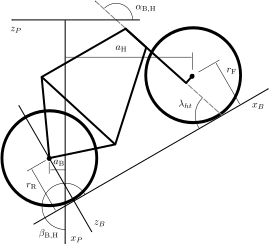
\includegraphics[width=0.8\onecolwid]{../../../figures/angles.pdf}
            \end{center}
            \rmfamily{
            The in- and out-of-symmetric plane moments of inertia were estimated by
            hanging the bodies as torsional and compound pendulums,
            respectively. We then estimated the period of oscillation by
            fitting a decaying oscillation function to a voltage signal from a
            rate gyro after the pendulums were perturbed. The period can then
            be correlated to the inertia.
            }
            \\
            \begin{center}
              \includegraphics[width=0.90\onecolwid]{../../../plots/PendFit/BrowserFrameCompoundFirst1.pdf}
            \end{center}
        \end{block}

\end{column}

% Spacer column
\begin{column}{\sepwid}\end{column} % empty spacer column

\begin{column}{\onecolwid}
  % Frequency Response
  \begin{alertblock}{Frequency Response}
    \small{\rmfamily{
    The steer torque to roll angle Bode plot reveals up to 15 dB variation
    among the bikes at 2 m/s and some variation in phase.
    }}
    \\
    \begin{center}
      \includegraphics[width=.85\onecolwid]{../../../plots/Bike/Bode/Tdel2phi.pdf}
      \\
      \includegraphics[width=.85\onecolwid]{../../../plots/BikeRider/Bode/Tdel2phi.pdf}
    \end{center}
  \end{alertblock}

  % References
  \begin{block}{References}
    \small{\rmfamily{
    \bibliographystyle{plain}
    \bibliography{bicycle}
    }}
  \end{block}
\end{column}
%\vskip2.5ex

% Last spacer column
\begin{column}{\sepwid}\end{column}			% empty spacer column

\end{columns}
}
%\end{frame}
\end{document}
